\documentclass[11pt,a4paper]{article}
\usepackage[top=3cm, bottom=3cm, left=2.5cm, right=2.2cm]{geometry} %geometry of page
\usepackage[hidelinks]{hyperref} %reference links
\usepackage{fancyhdr} %header and footer control
\usepackage{minted} %source code syntax highlighting
\usepackage{qrcode} %qrcode links
\usepackage{graphicx} %images
\usepackage{tikz} %diagrams
\usetikzlibrary{calc}

\linespread{1.3}
\emergencystretch 3em

% Set Header and Footer
\fancyhead{}
\fancyhead[L]{\textbf{Lab 5: Control system}}
\fancyhead[R]{d.s.brennan@sheffield.ac.uk}
\fancyfoot{}
\fancyfoot[L]{\thepage}
\fancyfoot[R]{MAC 233 Arduino Labs, School of MAC, University of Sheffield}

% Create Document
\begin{document}
\pagestyle{fancy}

\section*{Prerequisites}
This worksheet builds upon the Lab 4 worksheet. You will have needed to complete the Lab 4 worksheet before you can continue with this lab. Out of your Arduino pack, you will need: 1 Arduino, 1 A3144 hall effect sensor, 1 Servo, 1 LED, 1 $10K\Omega$ resistor, 1 $220\Omega$ resistor, and 8 jumper cables.

\section*{Objectives}
The Objectives of today's lab is to build a full control system; namely, using a hall effect sensor to determine if an Electronic Speed Controller (ESC) --- and associated motor --- should be powered up or down. While the system we build today is designed for an ESC and motor, we will be using a servo as a proxy. As mentioned in the Lab 3 worksheet, both an ESC and a servo operate the same way within the context of an Arduino; however, an ESC requires additional configuration outside the scope of an Arduino.

\section{Creating the circuit}
\label{sec:circuit}
There are three circuits needed for this worksheet, the first is for the hall effect sensor (HES), the second is for the visual display LED, and the third is for the ESC.\\
\noindent
\textbf{HES circuit}: Arduino +5V\textrightarrow\hspace{0.1em}HES left leg, Arduino GND\textrightarrow\hspace{0.1em}HES middle leg, Arduino Pin D2\textrightarrow\hspace{0.1em}HES right leg. HES left\textrightarrow \hspace{0.1em}$10K\Omega$ resistor\textrightarrow\hspace{0.1em}HES right legs.\\
\noindent
\textbf{LED circuit}: Arduino Pin D4\textrightarrow $220\Omega$ resistor\textrightarrow LED\textrightarrow Arduino GND.\\
\noindent
\textbf{ESC circuit}: Arduino +5V\textrightarrow Servo power cable, Arduino GND\textrightarrow Servo ground cable, Arduino Pin D9\textrightarrow Servo sensor cable.

\section{System Functionality}
\label{sec:functionality}
The basis of this system is the same as is described in Lab 4: \textit{creating a system with a hall effect sensor, so that whenever a magnet passes the field of the hall effect sensor, we turn on a LED}. The worksheet in Lab 4 walks you through how to do this through an \textit{interrupt} to record the time in milliseconds of when the hall effect value changed. In the `loop' function, if the time difference between the current time, and the last recorded hall effect interrupt time is less than 500 milliseconds, we turn on the light; otherwise, we turn it off.\\

\noindent
This worksheet simply expands that logic to include an ESC --- say connected to a motor on the back wheel of a bike. If the last recorded time of the hall effect interrupt is less than 1500 milliseconds, we slowly power up the ESC until it reaches maximum output. If at any point during the power up of the ESC, the last recorded hall effect interrupt drops outside that 1500-millisecond window, we power down the ESC.

\section{Changing the existing code}
Firstly, open your sketch from the Lab 4 worksheet into Arduino IDE. Once this is open, save the sketch under a new name (`File'\textrightarrow `Save As'). This will make sure you still have a copy of the sketch from Lab 4. The code changes required can be summed up into three sections: 1 - defining the ESC and required constants (global scope), 2 - setup the pins (`setup' scope), 3 - determine to power up or down the ESC (`loop' scope). While this is all the code required to meet the specification of the system, we will also be adding in some additional debug information, so you can see how the system is powering up the ESC.

\subsection{Defining the ESC}
The first thing we need is to include the ESC definitions and library to correctly control the ESC --- a servo is our case. We need to include the standard servo library, define a new `$ESC\_PIN$' on pin D9, define a 1.5-second maximum delay for the hall effect sensor, and define a new 1-second interval on how often to display a debug message.\\
\vspace{-1.75em}
\inputminted{arduino}{./src/1-define.txt}
\vspace{.75em}

\noindent
The next section of logic to include is two constant values that dictate the rate of increase and decrease of power to the ESC. The first constant sets that when we are powering up the ESC, we will increment the ESC output value by 0.5 every iteration of the `loop' function. The second constant sets that when we are powering down the ESC, we will decrement the ESC output value by 3.0 every iteration of the `loop' function. This gives us the facility to accelerate slowly but decelerate quickly.\\
\vspace{-1.75em}
\inputminted{arduino}{./src/2-esc-constants.txt}
\vspace{.75em}

\noindent
The last section of logic within the global scope is to create a variable to store when we last displayed the diagnostic message, the current power output to the ESC, and a reference to the servo library to control the ESC.\\
\vspace{-1.75em}
\inputminted{arduino}{./src/3-system-variables.txt}
\vspace{0em}

\subsection{Pins}
The code within the `setup' function is the standard code we have seen before: firstly we initialise any variables that don't have an initial value --- `$message\_previous\_time$' in our case, then we need to set up the ESC pin and library as we did in Lab 3.\\
\vspace{-1.75em}
\inputminted{arduino}{./src/4-servo.txt}
\vspace{0em}

\subsection{Powering the ESC}
The code within the `loop' function is new code that you haven't seen before, but it builds upon everything covered in previous labs. The first piece of code to add to your sketch is the code that determines if you should be powering up or powering down the ESC. We do this through a nested `IF ELSE' statement. \\

\noindent
The outer `IF' statement checks if the current time of the `loop' minus the last time the hall effect interrupt was recorded, is less than 1500 milliseconds. If this is true, we increment the ESC output value by the `step up' value, as long as the power output value wouldn't exceed the maximum of 180 --- if it does, we set it to the maximum value. If the outer `IF' statement was false --- the last interrupt wasn't recorded within the last 1500 milliseconds of the current `loop' time, we start to power down the ESC. We decrement the ESC power output value by the `step down' value, as long as the output value wouldn't go below the minimum 0 value --- if it does, we set it to the minimum value.\\

\noindent
The last line of code is to finally write the calculated output value to the ESC.\\
\vspace{-1.75em}
\inputminted{arduino}{./src/5-esc-power.txt}
\vspace{.75em}

\noindent
The last section of code is to help us understand what is going on with the system; however, before we can add this into our sketch we need to remove 1 line of code: `$Serial.println("Crank Active");$'. Once the above code has been removed, we can add the code in below which will print a diagnostic message every second to tell us what the current output power of the ESC is.\\
\vspace{-1.75em}
\inputminted{arduino}{./src/6-message.txt}
\vspace{-1em}

\section*{Try it out on your Arduino}
You now should be able to compile your sketch (`Sketch'\textrightarrow `Verify/Compile') and then upload to your Arduino (`Sketch'\textrightarrow `Upload'). You should now be able to pass the magnet across a side of the hall effect sensor, and every time you do, it should light up the LED, and your servo should start to power up. When you stop passing the magnet past your hall effect sensor, the servo will start to power down.\\

\noindent
Once you have a working sketch, try to expand your sketch to calculate the speed (Kmph) that the magnet is passing your hall effect sensor, and display the speed in your debug message. \textit{Hint: You will need to record the last two interrupt times.}

\pagebreak
\section*{Help}
If you are having issue compiling the project or don't understand where each section goes, you can see a complete version of the sketch with additional source code comments at \url{https://github.com/dsbrennan/mac-233-arduino-labs/blob/main/lab-5-control-system/lab-5-control-system.ino}.

\begin{center}
    \qrcode[hyperlink, height=3cm]{https://github.com/dsbrennan/mac-233-arduino-labs/blob/main/lab-5-control-system/lab-5-control-system.ino}
\end{center}

\vspace{2em}

\noindent
Additionally, if you are wondering how to wire up the circuit required for this lab on the breadboard, the electronic wiring diagram is below.

\begin{center}
    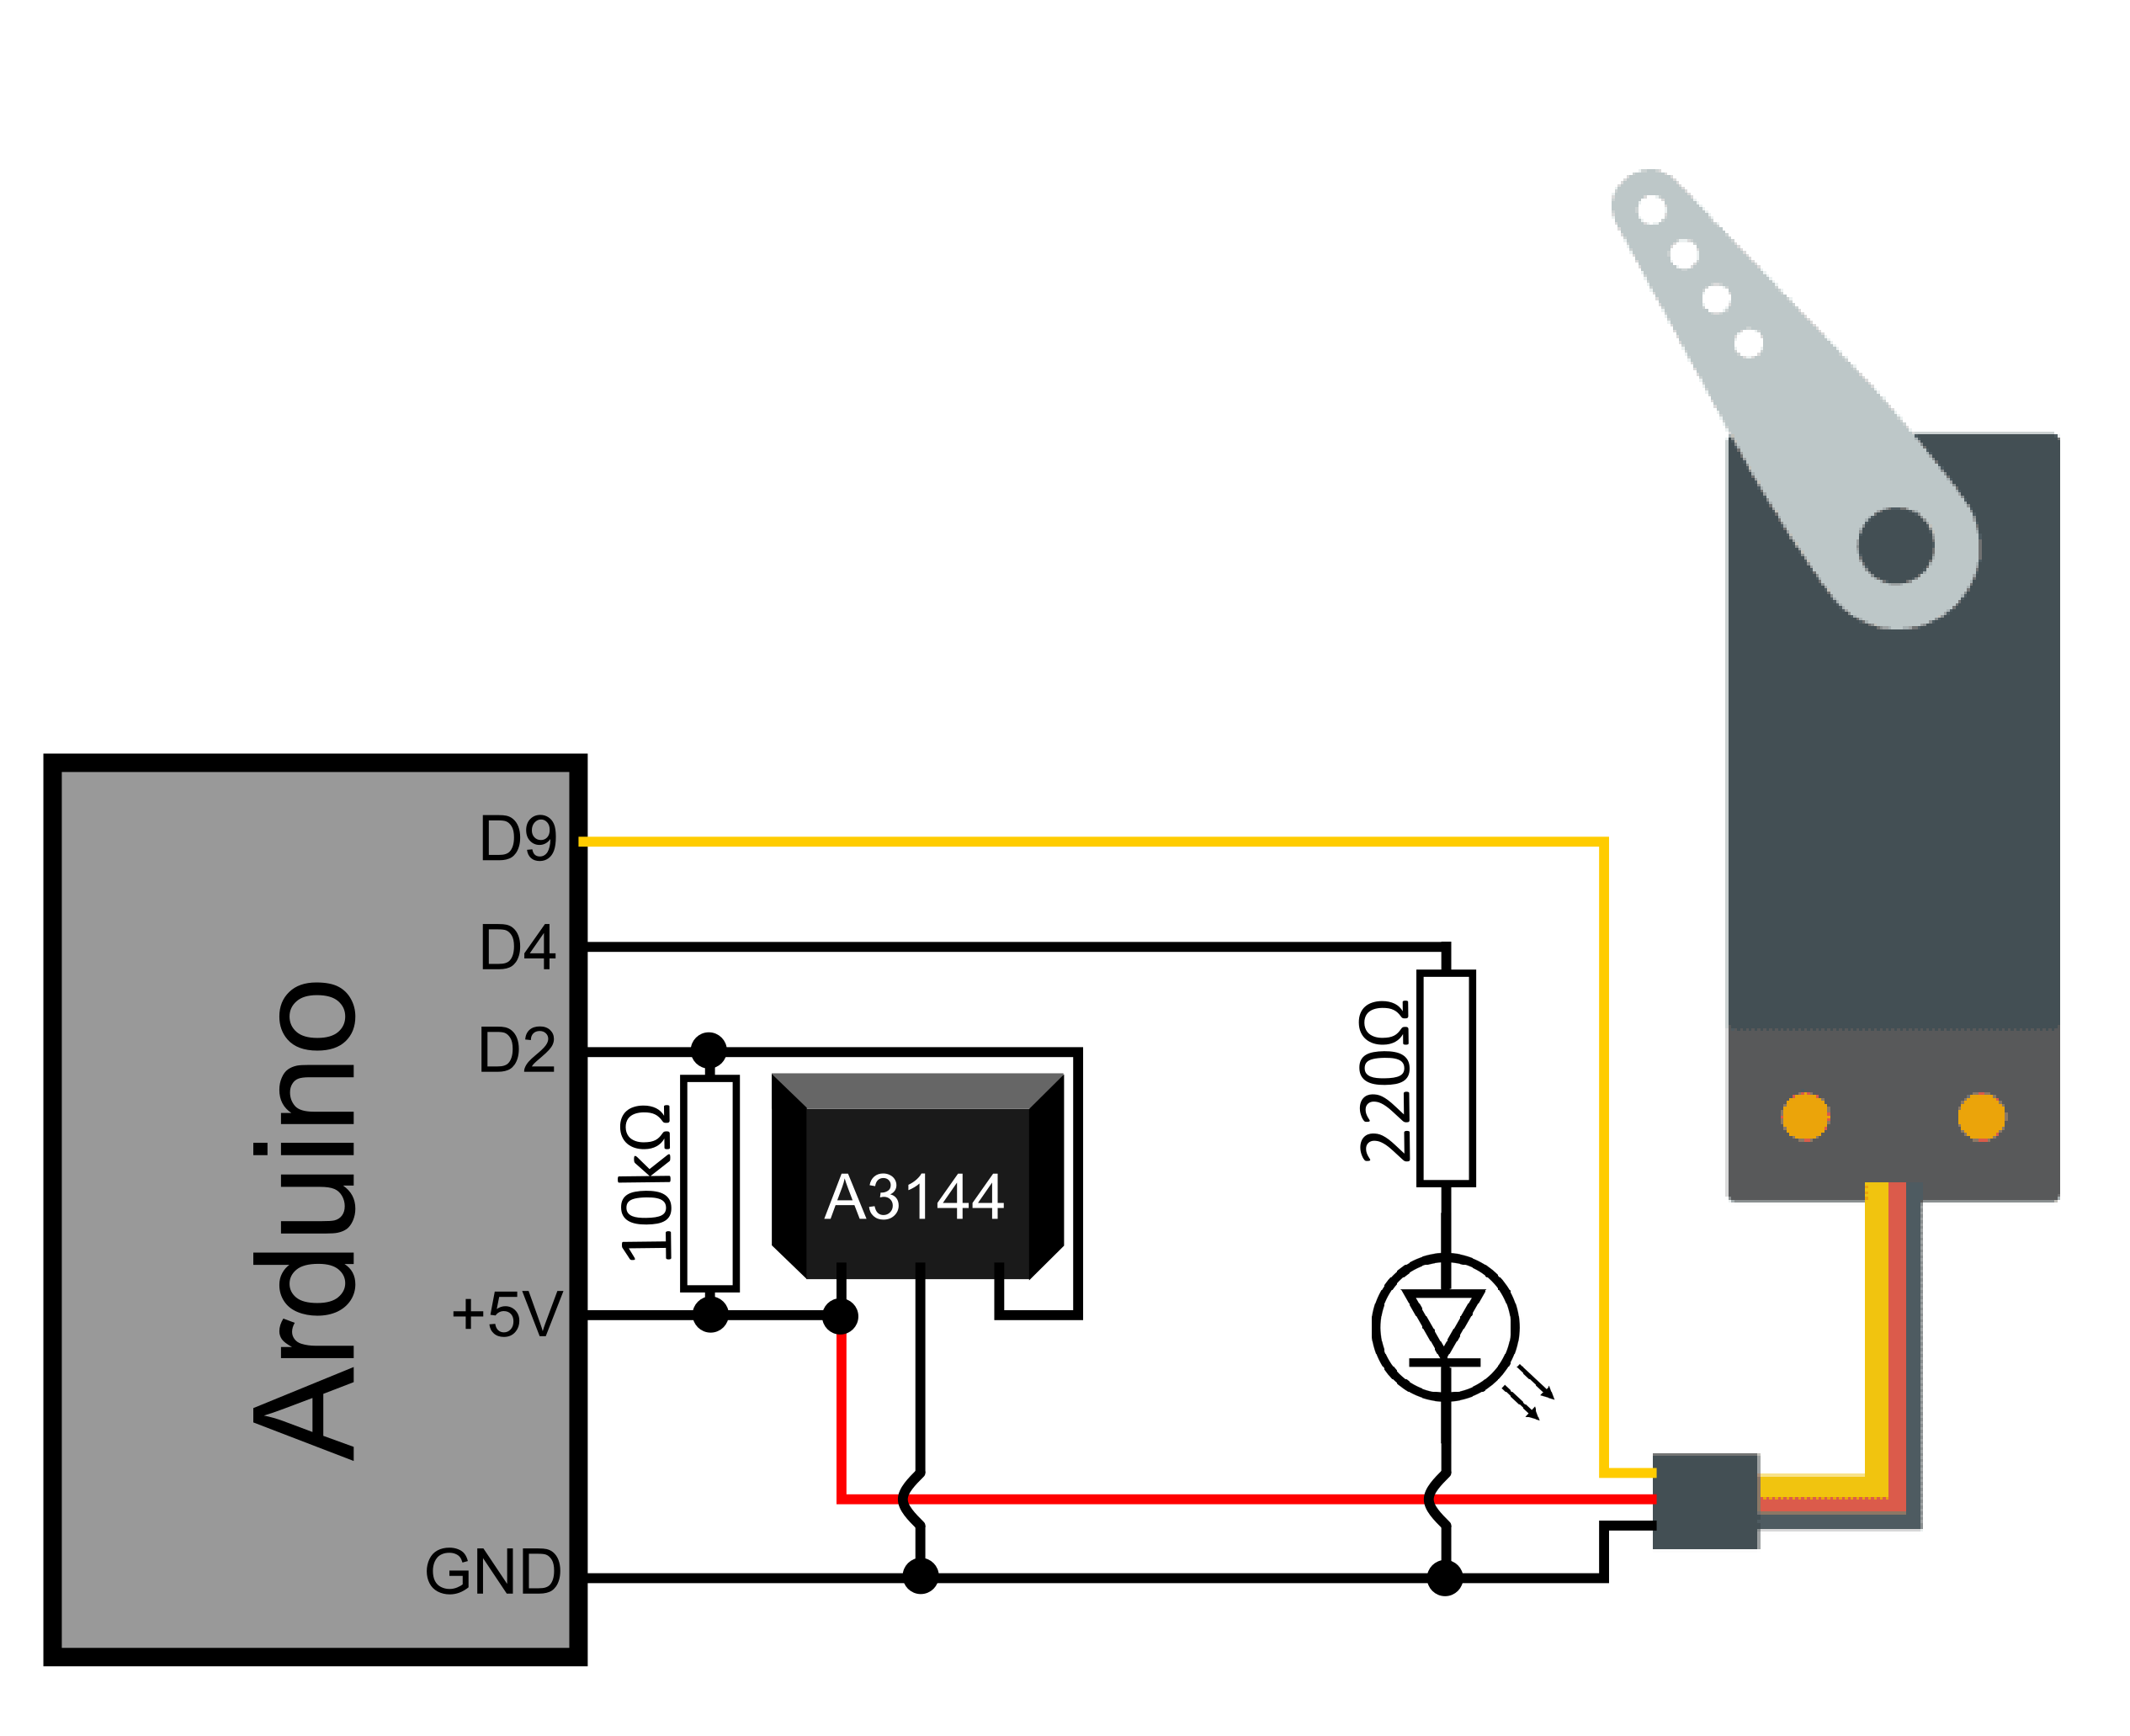
\includegraphics[width=.6\textwidth]{./images/wiring-diagram.png}
\end{center}

\end{document}